\subsubsection{Programación Unity Pro}
\begin{tcolorbox}[colback=blue!5!white,colframe=blue!75!black,title=Definición]
	Es una herramienta de configuración, programación y depuración de PLC de la empresa \textbf{Schneider Electric}.
\end{tcolorbox}

\paragraph{Guia}
Para generar la base del proyecto para trabajar, se debe descargar desde la página oficial e instalar el software Unity Pro XL y la librería DTM utilizada anteriormente en el software soMove. Una vez que esto está instalado se abre un nuevo proyecto y se configura como se muestra a continuación.
\begin{enumerate}
	\item Se selecciona el bastidor que se posee y los módulos (Figura \ref{fig:uni1}, (Figura \ref{fig:uni0}).
	
	\item 
\end{enumerate}
\hl{poner las figuras aparte}
\begin{center}
	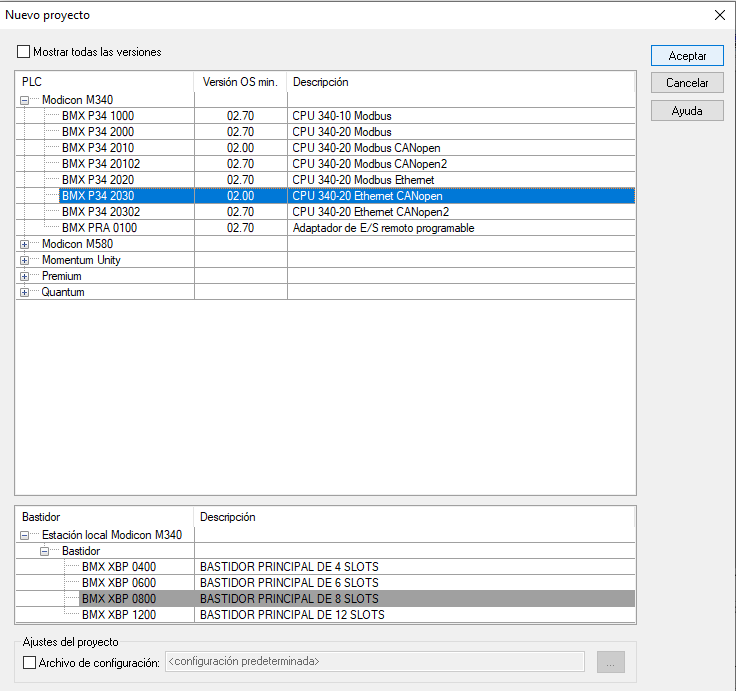
\includegraphics[scale=0.25]{unit1.png}
	\captionof{figure}{Elección del bastidor}
	\label{fig:uni1}
	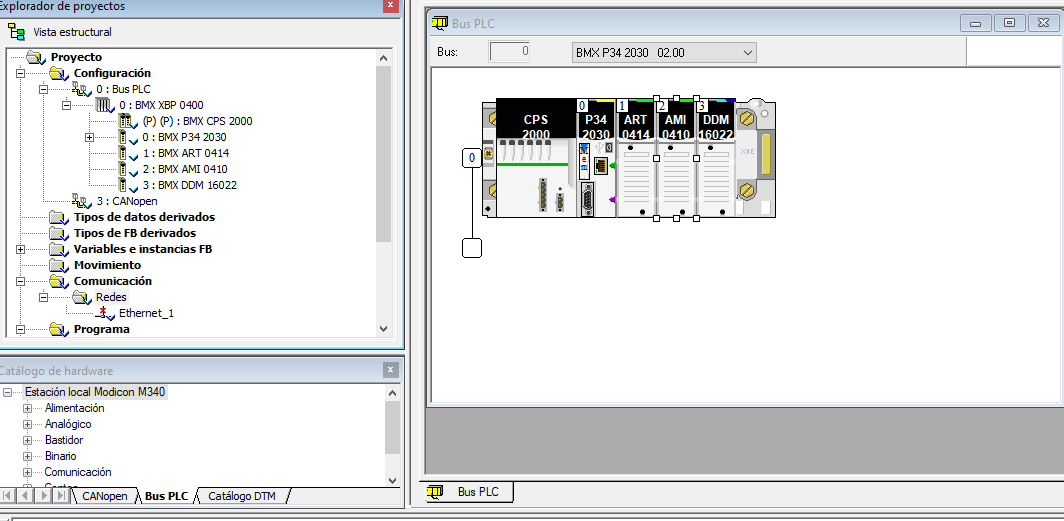
\includegraphics[scale=0.25]{unity1.png}
	\captionof{figure}{Módulos PLC}
	\label{fig:uni0}
\end{center}




\paragraph{Programa básico}
\newpage

